\documentclass[10pt,twocolumn]{article}

\usepackage{times}
\usepackage{fullpage}
\usepackage{graphicx}
\usepackage{epstopdf}

\begin{document}

\title{Efficient Virtualization on Embedded Power Architecture\textsuperscript{\textregistered} Platforms}
\author{}
\date{}
\maketitle
\thispagestyle{empty}

\maketitle
\begin{abstract}
  Power Architecture\textsuperscript{\textregistered} processors are popular and widespread on embedded systems, and such
  platforms are
  increasingly
  being used to run virtual machines\cite{embedded_virtualization, KVM_on_embedded_Power}. While the Power
  Architecture meets the
  Popek-and-Goldberg virtualization requirements for traditional trap-and-emulate
  style virtualization, the performance overhead of virtualization remains high.
  For example, workloads exhibiting a large amount of kernel activity typically
  show 3-5x slowdowns over bare-metal.

  Recent additions to the Linux kernel contain guest and host side paravirtual
  extensions for Power Architecture platforms. While these extensions improve performance
  significantly, they
  are guest-intrusive, non-portable and cover only a subset of all possible
  virtualization optimizations.

  We present a set of host-side optimizations that achieve comparable
  performance
  to the aforementioned paravirtual extensions, yet being
  guest-neutral. Our optimizations are based on adaptive binary translation.
  The only
  guest modification required by us is to include a guest-side virtual device driver
  to create a shared address space between the guest and the host.
  Unlike the paravirtual approach,
  our solution can optimize dynamically generated guest code, and gracefully
  handle self-referential and self-modifying code in the guest.
  We implement our ideas in a prototype based on Qemu/KVM.
  After our modifications, KVM can boot a Linux guest around 2.5x faster. Our solution
  provides equivalent performance to
  the paravirtual approach, without being guest-specific.
\end{abstract}
\section{Introduction}
Embedded devices based on Power Architecture processors are dominant for their
favourable power/performance characteristics. Virtualization on these platforms is
compelling for several applications including high availability (active/standby
configuration without additional hardware), in-service upgrade, and many
more\cite{embedded_virtualization, KVM_on_embedded_Power}. While newer Power
Architecture platforms
have explicit support for efficient virtualization\cite{freescale_embedded_hyperv, hwassists_hyperv}, a majority of
prevalent embedded devices run on older (and cheaper) Power Architecture platforms that use
traditional trap-and-emulate style virtualization\cite{popekgoldberg}. Efficient
virtualization is highly desirable on these platforms.

The current virtualization approach on Power Architecture platforms uses traditional
trap-and-emulate. The guest operating system is run unprivileged, causing each
execution of a privileged
operation to exit into the hypervisor. For guest workloads executing a large number
of privileged instructions, these VM exits are a major performance
bottleneck. Table~\ref{tab:kvm_performance} lists the performance of vanilla Linux/KVM
on a few common workloads, comparing them with bare-metal performance.
For example, a guest Linux boot takes almost 5x longer when run virtualized.

The poor performance of simple trap-and-emulate style virtualization has led to
the inclusion of paravirtual extensions in the Linux kernel on both
guest and host sides for Power Architecture platform\cite{pvpower}. The paravirtual extension in the guest
rewrites the guest (binary) kernel
code at startup time to replace most privileged instructions with
hypervisor-aware unprivileged counterparts.
At guest startup, the guest creates a shared address space with
the host through a {\em hypercall}. This shared address space
is used by the hypervisor to store guest state information, which
is accessible to the guest without incurring a trap.
Table~\ref{tab:kvm_performance} lists KVM performance after enabling paravirtual
extensions in the guest and the host. The performance improves significantly over
unmodified KVM.

The paravirtual approach has shortcomings. Firstly, extensive guest
modifications are required, which makes the optimizations highly Linux specific.
Secondly, this approach
cannot optimize dynamically generated/loaded code (e.g., loadable modules) because
all translation is done at kernel startup time.
The paravirtual approach also
fails in presence of self-referential and
self-modifying code in guest, as binary rewriting is done only
once at startup time, and other parts of guest kernel may be unaware
of this rewriting operation.
The Linux guest paravirtual extensions rely on such code not being present in the
kernel. These constraints are ungraceful, and hard to maintain.

We propose a host-side adaptive binary translation mechanism to optimize guest
privileged instructions at runtime. Our approach is more general than
the paravirtualization approach; we can optimize dynamically
generated/loaded code, and can gracefully handle
self-referential and self-modifying
code in the guest. We require minimal guest
modifications (in the form of a device driver to setup shared address spaces)
and achieve
comparable performance to the paravirtual approach.
The second-last column in Table~\ref{tab:kvm_performance} summarizes the performance results of
our host-side binary translation approach.

Our host-side virtualization optimizations are based on adaptive binary
translation. On observing a large number of VM exits by a guest instruction, we translate
that instruction {\em in-place} to directly execute the corresponding
VMM logic (thus avoiding an exit). In doing so, we directly modify the guest's
address space. This is in contrast to a {\em full} binary translation approach
that translates the entire guest code
(e.g., VMware's x86-based binary translator\cite{adams:asplos06}). Our approach is
simpler and incurs less overhead than full binary
translation approaches. We compare the two approaches in more detail in
Section~\ref{sec:comparison_with_full_bt}.

Modifying the guest's address space has obvious pitfalls.
Firstly, we must ensure correctness in presence
of arbitrary branches in the code. For example, it would be incorrect if the guest
could potentially jump to the middle of our translated code.
%We rely on the fixed-length
%word-aligned nature of Power Architecture instructions to achieve correctness.
To ensure correctness, we replace a privileged guest instruction
by at most one translated instruction in the guest's address space. Because instructions
are fixed length and word aligned on Power Architecture platform, this ensures that
there can never be a branch to the middle of our translated
code. Any branch could only reach either the beginning or the end of our
replacement instruction.

Not all guest privileged instructions can be emulated by just one
replacement instruction.
Such instructions are instead replaced with a branch to a code
fragment in a host-managed translation cache. This branch is implemented as a
single instruction in the guest's address space, and the translation
cache is allocated in host's address space. We provide a mechanism for the guest
to directly access the translation cache in host's address
space (details in Section~\ref{sec:bintrans}).

The second challenge with in-place guest modification is dealing with
self-referential and self-modifying guest code. We maintain correctness by 
marking the pages containing the modified instructions {\em execute-only}. This
causes the hardware to trap into the VMM on any guest read/write access to the
modified code. We call this mechanism {\em read/write tracing}.

Finally, read/write tracing can cause a large number of
page faults, especially due to false sharing. The problem is
exacerbated on embedded Power Architecture platform, where OS typically uses
huge pages to reduce TLB pressure. We found that such page faults can
significantly reduce performance.
We implement two important optimizations to address this problem, namely
{\em adaptive page resizing} and {\em adaptive data mirroring}.

In summary, this paper presents an efficient host-side optimization solution for
Power Architecture virtualization. Our approach is based on in-place binary translation,
and maintains guest correctness in presence of self-referential and self-modifying
guest code.
The paper is organized as
follows. Section~\ref{sec:performance_char} characterizes the performance of
KVM on Power Architecture platform and discusses the typical sources of overhead.
Section~\ref{sec:bintrans} discusses our in-place binary translation approach.
We discuss read/write tracing and our optimizations to make
it efficient in Section~\ref{sec:tracing}.
Section~\ref{sec:results} presents our experiments and results, and
finally Sections~\ref{sec:discussion}-\ref{sec:conclusion} conclude.

\section{Performance Characterization of KVM on Power Architecture Platforms}
\label{sec:performance_char}
We perform our experiments on Linux/KVM running on Freescale P2020
embedded Power Architecture platform.
On our test platform, the virtualization overheads
of trap-and-emulate style virtualization can be up to 15x for compute-intensive
workloads executing a large number of privileged
instructions (Table~\ref{tab:kvm_performance}). The primary source of
overhead are VM-exits due to guest privileged instructions.
Table~\ref{tab:priv_opcodes} lists the most executed privileged
opcodes and briefly explains their semantics.
Figure~\ref{fig:opcode_exit_fraction} shows the percentage of exits caused
due to each opcode. Only five opcodes result in more than 80\% of exits on all
three benchmarks. Table~\ref{tab:exitcount_linuxboot} presents the frequency
profile of VM exits on the Linux boot benchmark in more detail.

We next profile the number of distinct program counter (PC) values that
cause exits. Figure~\ref{fig:pc_profile} shows a histogram on the number
of distinct PC values and the frequency of exits on them.
Table~\ref{tab:pcexits_linuxboot} presents the exit profile of different
PCs in more detail for the Linux boot benchmark. For example, around 92\% of all
exits are caused by only 93 distinct PCs for guest Linux boot. These
measurements confirm that
binary translating
only the most frequently executed opcodes/PCs is likely to produce large
improvements.

\begin{table}[!b]
\centering
     \begin{tabular}{|l | p{5cm} |} \hline
       Opcode \verb, , & Description \\ \hline
       {\tt mfmsr} & Move from machine state register \\ \hline
       {\tt mtmsr} & Move to machine state register \\\hline
       {\tt mfspr} & Move from special purpose register \\\hline
       {\tt mtspr} & Move to special purpose register \\\hline
       {\tt wrtee(i)} & Write MSR External Enable  \\\hline
       {\tt rfi} & Return from Interrupt \\\hline
       {\tt tlbwe} & Writes a TLB entry in hardware\\\hline
       \hline
       Exception \verb, , & Description \\ \hline
       {\tt dtlbmiss} & Page fault on data due to TLB not present\\    \hline
       {\tt itlbmiss} & Page fault on instruction due to TLB not present\\    \hline
       {\tt dsi} & Page fault due to insufficient privilege\\\hline

     \end{tabular}
\caption{\label{tab:priv_opcodes} Sources of VM Exits: Opcodes and Exceptions}
\end{table}

\begin{figure}[!htb]
\centering
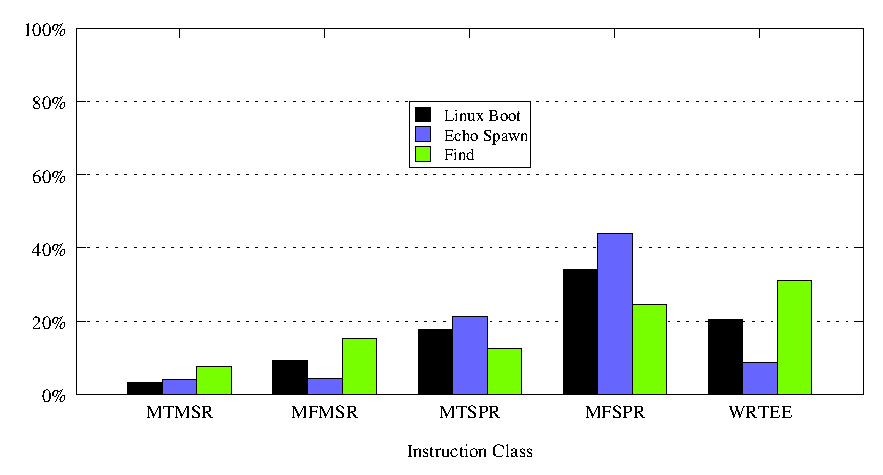
\includegraphics[scale=0.5]{exit_count.eps}
\caption{\label{fig:opcode_exit_fraction}Main sources of VM exits}
\end{figure}

\begin{table}[!b]
\centering
     \begin{tabular}{lcc} \hline
       Instruction class  & Exit count & \% of total exits  \\ \hline
       {\tt mfspr} & 4484245 & 33.8  \\
       {\tt wrtee} & 2792109 & 21.1  \\
       {\tt mtspr} & 2307647 & 17.4  \\
       {\tt mfmsr} & 575302 & 9.5 \\
       {\tt rfi} & 413847 & 4.3 \\
       {\tt mtmsr} & 391813 & 3.1 \\
       %TLBWE & 247282 & 2.9 \\
       %DTLBREAL & 241070 & 1.8 \\
       %ITLBREAL & 241070 & 1.8 \\
       {\tt dtlbmiss} & 198239 & 1.5 \\
       {\tt itlbmiss} & 192046 & 1.4 \\
       \hline
     \end{tabular}
\caption{\label{tab:exitcount_linuxboot}Main sources of VM exits and their frequency on guest Linux boot (refer Table~\ref{tab:priv_opcodes} for semantics of these opcodes)}
\end{table}

\begin{figure}[!htb]
\centering

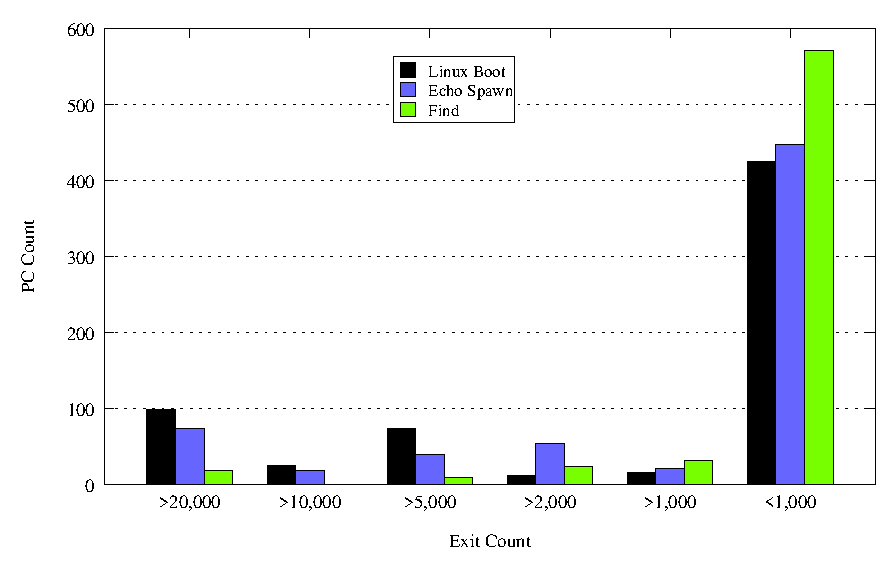
\includegraphics[scale=0.5]{pc_count.eps}
\caption{\label{fig:pc_profile}Exit Profile of Different Guest PCs for three different macrobenchmarks}
\end{figure}

\begin{figure}[!htb]
\centering

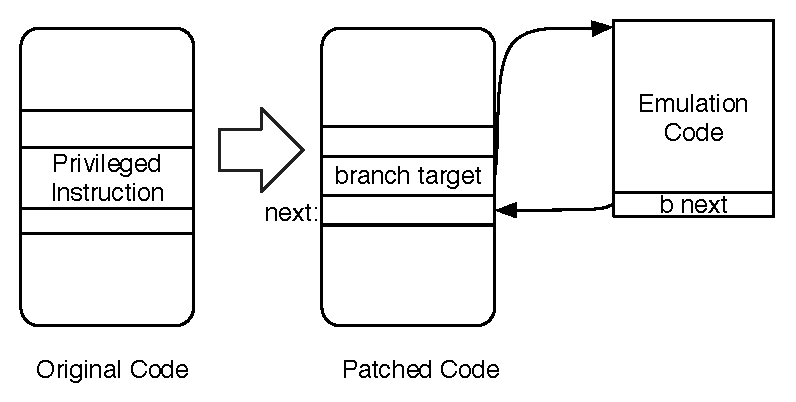
\includegraphics[scale=0.5]{txcache.eps}
\caption{\label{fig:txcache}Figure showing patching of multiple instructions with {\tt branch} instruction.}
\end{figure}

\begin{figure}[!htb]
\centering
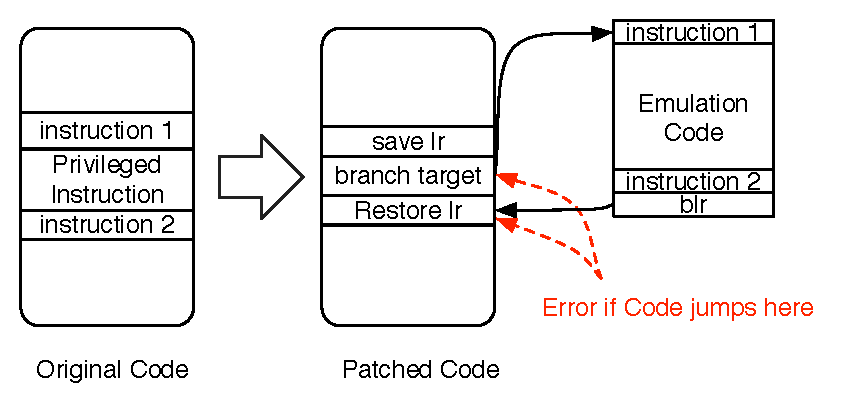
\includegraphics[scale=0.5]{multiple_ins_patching.eps}
\caption{\label{fig:multiple_insns_patching}Figure showing patching of multiple instructions using {\tt bl} instruction. This approach fails in presence of arbitrary guest jumps.}
\end{figure}



\begin{table}
\centering
     \begin{tabular}{lcc} \hline
       Exits count  & PC count & \% of total exits  \\ \hline
       $>$20000 & 93 & 91.9  \\
       $>$10000 & 23 & 3.1  \\
       $>$5000 & 68 & 4.2  \\
       $>$2000 & 12 & 0.3 \\
       $>$1000 & 17 & 0.2 \\
       $<$1000 & 299 & 0.2 \\
       \hline
     \end{tabular}
\caption{\label{tab:pcexits_linuxboot}PCs responsible for VM exits on guest Linux boot}
\end{table}


\begin{table*}
\centering
      \begin{tabular}{|l@{}| l@{}|p{3.8cm} | r r r r r|} \hline
        S.No.\verb, ,&  Benchmark\verb, ,& Description  & Bare-metal \verb, ,& {\tt KVM} \verb, , & {\tt KVM-PV} \verb, ,& {\tt KVM-BT}& Speedup \\ \hline

     &&& \multicolumn{5}{c|}{ Running Time in $sec$}\\\cline {4-8}  
      1&  Linux Boot& linux boot & 6.5	&	30.03	&	11.79	&	12.24 & 2.5x \\ \hline
      2& Echo Spawn	& Spawning a large number of echo processes&1.4	&	21.34	&	6.5	&	7.26& 2.9x \\\hline
      3& Find	& find / -name temp & 0.39	&	1.89	&	0.67	&	0.71 & 2.7x\\ \hline
	   \multicolumn{3}{|c|}{ lmbench microbenchmarks }& \multicolumn{5}{c|}{Latency in $msec$}\\  \hline

4	&	syscall	&	 measures time to write one word to /dev/null	&	0.000	&	0.020	&	0.003	&	0.003 & 6.7x	\\	\hline
5	&	stat	&	 measures the time to invoke the stat system call	&	0.003	&	0.033	&	0.006	&	0.007& 4.7x	\\	\hline
6	&	fstat	&	time to invoke fstat system call on open file 	&	0.001	&	0.021	&	0.004	&	0.004&5.3x	\\	\hline
7	&	open/close:	&	 time to open a temporary file for reading and closing it immediately 	&	0.006	&	0.067	&	0.013	&	0.014&4.8x	\\	\hline
8	&	sig hndl	&	 time to install a signal handler	&	0.001	&	0.024	&	0.004	&	0.004	& 6x\\	\hline
9	&	pipe 	&	 round trip latency to pass a word from process A to process B and back to A	&	0.014	&	0.164	&	0.032	&	0.034&4.8x	\\	\hline
10	&	fork	&	 fork and exit 	&	1.084	&	6.641	&	1.640	&	2.061&3.2x	\\	\hline
11	&	exec	&	 fork, exec and exit	&	3.065	&	20.543	&	6.254	&	7.533&2.7x	\\	\hline
12	&	sh	&	 fork, exec sh -c and exit	&	6.645	&	45.164	&	13.842	&	16.327&2.8x	\\	\hline



        \hline
      \end{tabular}
\caption{\label{tab:kvm_performance}Performance comparison of bare-metal, unmodified KVM, KVM-paravirtual, and our (KVM-BT) approach. The details of
the benchmarks, our test system, and the various KVM variants is discussed in Section~\ref{sec:results}. The last column computes the speedup of {\tt KVM-BT} over {\tt KVM}.}
\end{table*} 
%\begin{table}[!b]
%\centering
%\caption{Performance of Base KVM}
%     \begin{tabular}{lcc} \hline
%       Benchmark  & Performance (\% of bare-metal) \\ \hline
%       Linux Boot & 21.7 \\
%       Echo Spawn & 6.4 \\
%       Find & 20.6 \\
%       \hline
%     \end{tabular}
%\label{tab:kvmperformance}
%\end{table}

%\begin{table}[!b]
%\centering
%\caption{Tracing overhead optimizations - Approaches}
%     \begin{tabular}{|l | p{5cm} |} \hline
%       Approach \verb, , & Description \\ \hline
%       Static-TLB & In-place Binary Translation and Read/Write Tracing with static TLB configuration\\ \hline
%       Adapt-DM & Avoiding Read Page Faults by copying data and translating faulting instructions  \\\hline
%	   Adapt-PR & Adaptive Page Resizing  \\\hline
%
%     \end{tabular}
%\label{tab:diff_approaches}
%\end{table}

\section{In-place Binary Translation}
\label{sec:bintrans}
We monitor PCs causing a large number of VM exits and binary translate them to
avoid these exits.
We translate guest instructions in-place. These translations could potentially
require code fragments involving multiple instructions. To ensure correctness, we
must place these code fragments in {\em reserved} space (i.e., not accessed by
guest for other purposes). We require the guest to explicitly reserve this space
and inform the host through a hypercall. The first step of our
binary translation solution is to setup a shared address space between
the guest and the host and we discuss this in the following
subsection.
\subsection{Shared Host-Guest Address Space}
\label{sec:sharedspace}
The guest reserves some pages in it's address space to store the
binary translator's translation
cache. The guest also reserves some pages to store it's emulated registers.
Both the translation cache and guest's emulated registers are maintained by
the host. Hence the host must also have access to these pages, and hence these
are {\em shared address spaces}.

We require the guest to reserve these pages at startup and inform the host about
them using a hypercall.
This is the only guest modification we require.
We implement this page reservation
and hypercall as a virtual guest device driver (similar to the ``tools'' mechanism
used in many virtualization solutions). We envisage mechanisms to setup
such shared address spaces using well-known standards for device
discovery (e.g., ePAPR\cite{ePAPR}) in future.
We require 75 SLOC changes in a Linux guest to implement this mechanism.
%This is
%significantly less than the 1100 SLOC required by the Linux paravirtual
%extensions.

In our current implementation, two distinct address ranges are reserved by the
guest for our BT optimizations.
The first one is a 4KB page with guest read/write privileges
to store guest's emulated registers.  The second address range is 32KB long
with guest execute privileges to store the translation cache.

These shared address spaces also have placement constraints. For easy direct
addressing, we place the 4KB page (containing guest's emulated registers) at
the top of guest's virtual address space (at {\tt 0xfffff000}). This is important 
because direct memory-addressing modes on Power Architecture platform specify only 16-bit
addresses. For absolute addressing, this implies that the memory
address must lie in either
the lower 32KB ({\tt 0x00000000-0x00007fff}) or higher
32KB ({\tt 0xffff8000-0xffffffff}) of the virtual address space. Because the lower
addresses are reserved for user applications on Linux, we use the higher addresses.

The second shared address range to store the translation cache, also has placement
constraints. This execute-only space must be reachable
by a direct branch instruction from the guest code. A direct branch instruction
in Power Architecture ISA specifies a 26-bit
word-aligned address. The branch target addressing is either PC-relative
or absolute. This implies that the translation cache could be
in one of the following regions: {\tt 0x0000000-0x00ffffff}, {\tt 0xff000000-0xffffffff},
or within a $\pm$32MB distance of any instruction in guest's kernel code sections.
Also, as we explain in the
next section (Section~\ref{sec:bintrans}), the code in the translation cache must
be able to branch
back to the guest's code (to the instruction following the translated instruction).
Because guest's code could be arbitrarily placed, this constrains the translation
cache to be within $\pm$32MB distance of any instruction in
guest's kernel code section.

The guest reserves a 32KB execute-only space for the
translation cache within 32MB of the kernel's code
section. Given that kernel code sections are small (typically 5-6MB),
this constraint is usually easy to satisfy. If the execute-only
pages happen to lie beyond 32MB distance of a privileged instruction, that
instruction is precluded from being optimized. Other instructions that lie
within 32MB of the translation cache can still be optimized.

\subsection{Translation of Privileged Instructions}
Some privileged instructions can
be emulated by single-instruction translations. For example, {\tt mfmsr} is translated
to a {\tt load} instruction to the address of the emulated {\tt msr}
register in the shared read/write page. Other opcodes which can be
translated to single instructions are {\tt mfmsr}, {\tt mfspr} and {\tt mtspr}.
These opcodes requiring single-instruction translations cause the bulk of
privileged exits in common workloads (refer Figure~\ref{fig:opcode_exit_fraction}).
We call the privileged instruction
that was patched, the {\em patch-site}. 

Other privileged opcodes require translation to multiple instructions.
For such opcodes, we store the emulation code in the translation cache, and
patch the original instruction with a {\tt branch} instruction to jump to it's
emulation code. The emulation code in the
translation cache is terminated
with another branch {\em back} to the instruction following the patch-site
(see Figure~\ref{fig:txcache}). Because each patch-site requires a different
terminating branch instruction, a new translation is generated for
each patch-site.

%We use Power Architecture's unconditional direct {\tt branch} opcode to jump to the
%translation cache from the patch-site. The {\tt branch} opcode specifies a 24-bit
%branch offset, with either absolute or relative addressing. This constrains us
%to place the emulation code either within a 24-bit distance of the patch-site (i.e.,
%$\pm$16MB) or in the top or bottom 16MB of the guest's virtual address
%space (see Figure~\ref{fig:branchtargets}). We ensure this by mapping the shared
%page containing our translation cache within $\pm$16MB of the kernel's code
%section (as also mentioned in Section~\ref{sec:sharedspace}). XXX Discuss loadable
%modules and how they are handled.

This branch back to the instruction following the patch-site is
the primary reason behind constraining the translation cache to lie within
$\pm$32MB of the patch-site.
We investigated another possibility to avoid this constraint on the placement
of translation cache. Instead of using a direct {\tt branch} opcode, we used
the {\tt bl} opcode to jump to the translation cache. The {\tt bl} opcode is
identical to the {\tt branch} opcode, except that it additionally stores the
address of the following instruction in the link register {\tt lr}. This instruction
is meant to implement function calls (return address stored in {\tt lr}).
The {\tt bl} instruction
allows greater flexibility in the placement of translation cache. For example, it is
now possible to place the translation cache in the top 32MB of the address
space ({\tt 0xfe000000-0xffffffff}) and use absolute addressing for the {\tt bl}
instruction. For the branch back, we can simply use the {\tt blr}
instruction (branch to the address in {\tt lr}). {\tt blr} allows specification
of a full 32-bit address in {\tt lr} and can potentially jump anywhere in the
address space.
This solution however
clobbers the {\tt lr} register, which can deviate guest's behaviour.
We next tried saving/restoring the
{\tt lr} register at the patch-site before/after branching to the emulation code.
To do this, we patched not just the privileged instruction but also 1-2
surrounding instructions (see Figure~\ref{fig:multiple_insns_patching}). The
surrounding instructions are made part of the emulation code to preserve
guest behaviour. This can
be done safely only if the surrounding instructions are not control-flow instructions.

This {\tt bl}-based solution works correctly for emulation of the privileged opcode.
However, if the guest ever jumps to one of the surrounding instructions (which we
have replaced), the guest will behave incorrectly.
Because it is practically impossible to predict all possible branch targets at
translation time (due to presence of indirect branches), we discarded this potential
solution.

The hypervisor maintains the state of the translation cache in
a hash table indexed by the PC value of current patch-sites. Each hash table
entry stores patch-site PC, the patch-site's original contents,
the location of the corresponding emulation code in the shared page, and other
information useful
for cache replacement. In our implementation, we use the FIFO cache replacement policy
for it's simplicity and high performance.
\section{Read/Write Tracing}
\label{sec:tracing}
Changing instructions in the guest address space can cause
inconsistencies if the guest tries to read or write it's own code.
For this reason, we protect the pages containing patch-sites with hardware
page-protection bits. Embedded Power Architecture platforms provide three {\tt rwx}
protection bits per page for both user/supervisor privilege levels. Using these
bits, we can mark a guest page containing a patch-site
execute-only in user mode. This allows the
execution of an instruction on this page to proceed uninterrupted,
but any read or write access causes a page fault (and a VM exit).
On a page fault, the hypervisor
emulates the faulting instruction in software. We call this
method memory read/write tracing (similar to VMware's memory write tracing
on x86\cite{adams:asplos06}).

We implement software emulations of memory instructions in KVM. There are 36
different memory opcodes in Power Architecture ISA that need to be emulated.
For read instructions, we simply return the original contents of the memory
address in the appropriate destination
operand. The original contents may be obtained either from the present guest
page (if the address does not intersect with a patch-site), or from the hypervisor's
hash table (if the address matches a patch-site), or both.
For write instructions, if the memory address (and length) intersects with a patch-site,
we invalidate and free the corresponding translation cache
entry and replace the guest page with it's original contents before
re-executing the instruction. If the memory address does not intersect with a
patch-site, we simply perform the equivalent write operation to the guest's memory.

The overhead of read/write tracing depends on the number of accesses by the guest
to it's pages containing kernel code. For a Linux guest, we found that this overhead
can be quite significant.
Much of this overhead is due to false sharing. For example, a large number of page
faults occur because guest kernel data often resides on the same page as
guest kernel code. The problem becomes worse with increasing page size. Linux
on embedded
Power Architecture platform uses huge pages for kernel code/data to minimize
TLB pressure, causing our tracing mechanism to result in a huge number of page
faults. We call these {\em tracing page faults}.

We implement two optimizations to reduce tracing page faults. Our first optimization
adaptively resizes the guest's pages to reduce false sharing.
Our second optimization adaptively
mirrors guest data (which is causing a large number of faults) to reduce the number
of page faults caused by read accesses (which is the common case). For the second
optimization we also translate the faulting instruction to access the mirrored data.
We discuss both optimizations in detail below.

\subsection{Adaptive Page Resizing}
Typical TLB sizes on embedded Power Architecture processors are small.
For example, the software-managed TLB on our test system is a combination of a 16-entry
fully-associative cache of variable-sized page table entries
and a 512-entry 4-way set-associative fixed-size (4KB) page table entries.
A faster L1 TLB lookup cache is implemented in hardware, and all invalidations
to maintain consistency with the software-programmed L2 TLB are done automatically.
The variable-pagesize TLB cache supports 11 different page sizes: 4K, 16K, 64K,
256K, 1M, 4M, 16M, 64M, 256M, 1G, and 4G. Further a page of size $S$ must be $S$-byte
aligned in physical and virtual address spaces.

The hypervisor traps guest's accesses to the TLB, and creates appropriate
{\em shadow TLB entries}. These shadow entries are loaded into hardware
while the guest is
running. This mechanism is similar to the hardware-managed shadow page
tables used in x86\cite{adams:asplos06}. The guest cannot directly access the shadow
TLB entries, as guest's accesses to the TLB entries are trapped and emulated by
the hypervisor. This allows the hypervisor full flexibility in choosing the
size and privileges of it's shadow TLB entries. For example, the hypervisor
can setup multiple shadow TLB entries, to shadow a single guest TLB entry representing
a larger page.
To minimize TLB pressure, the hypervisor typically uses
one shadow TLB entry per guest TLB entry. For example, if the guest uses 4MB pages,
then the shadow TLB will also have corresponding entries for 4MB pages. We
implement read/write tracing by disabling read/write privileges in the shadow TLB entry.

Most operating systems use huge pages (using the variable pagesize TLB cache)
for the kernel to
reduce TLB pressure. The fixed pagesize TLB cache (containing mappings for 4K pages) is
made available primarily for user programs. For example, our Linux guest
uses just one 256MB TLB entry mapping all its kernel code and data.
Disabling read/write privileges from this TLB entry predictably causes an unacceptably
large number of page faults (every kernel data access becomes a page fault).

We resize shadow TLB entries to deal with this overhead of page faults due to read/write
tracing. After patching a privileged guest instruction, if we notice
a high number of tracing page faults on that page, we {\em break} the page into
smaller fragments (and the corresponding TLB entry into smaller TLB entries).
After breaking,
we only mark the
TLB entry containing the patch-site execute-only, and leave the remaining
unmodified.
To minimize false sharing, we keep the
size of the page containing the patch-site as small as possible, without
adversely effecting performance. All other pages created by this fragmentation
are sized
as large as possible, to minimize
the overall number of TLB entries. While smaller pages reduce false sharing, they
also result in increased TLB pressure.

After fragmentation of a large page, if we still notice a high number of page faults
on the smaller page (which cannot be broken further), we remove all patch-sites
on that page and re-instate read/write privileges on it. The decision on
whether to remove the patch-sites on a page, depends on the tradeoff
between the number of privileged-instruction exits and the number of
tracing page faults on that page.

Breaking a large page potentially creates
many smaller pages due to alignment restrictions.
For example, if the kernel has mapped
itself using a 256MB page at virtual address (0xc0000000,0xcfffffff), and a
patch is to be applied at address 0xc0801234, and we have decided to break
the patch-site page into a 4MB page, the new set of TLB entries will be for
addresses
(0xc0000000,0xc07fffff);(0xc0800000,0xc0bfffff);
(0xc0c00000,0xc0ffffff);(0xc1000000,0xc1ffffff);
(0xc2000000,0xc3ffffff);(0xc4000000,0xc7ffffff);
(0xc8000000,0xcfffffff). Notice that each page of size $S$ is $S$-byte
aligned.

We use the following fragmentation policy. On
observing a high number of tracing page faults (we use a threshold of 10000 faults in
100ms) on a page, that page is broken such that all patch-sites on that page
belong to 64KB pages. We do not break pages to smaller than 64KB to
limit TLB pressure. We periodically monitor the number of page faults on
each fragment. If we find that the number of page faults on a 64KB page is still high,
we remove all patch-sites and the trace on that page (based on the trade-off
between privileged-instruction exits and page faults, as discussed above).
Further, if we find that neighbouring pages have identical {\tt rwx} privileges
as a result of the above algorithm,
we opportunistically merge them into a larger page to reduce TLB pressure. We perform
these periodic checks every 100ms.

Adaptive page resizing significantly reduces the number of page faults. For
example, a Linux guest boots in 13.29 seconds (as opposed to 30.03 seconds on
unmodified KVM) with in-place binary translation
and adaptive page resizing for read/write tracing. Without adaptive page resizing,
the guest livelocks at boot time due to the large number of
page faults. A detailed study of the performance tradeoffs is presented in
Section~\ref{sec:results}.

\subsection{Adaptive Data Mirroring}
After implementing adaptive page resizing,
we still observed 10-20\% performance overhead due
to tracing page faults. We found that a major cause of these page faults were
read accesses to function dispatch tables and exception handler tables which were
colocated with kernel code. Often these tables share
the same 64KB region as the privileged kernel code accessing them, rendering our
adaptive page resizing algorithm ineffective on these accesses.

We avoid these faults by dynamically monitoring such page faults, adaptively
copying the data being accessed to host's shared address space, and
translating the instructions accessing this data to access from the new location.
This optimization prevents future page faults on this data.

We perform this optimization if the number of tracing page faults
due to a certain read-access instruction exceeds a threshold (we use a threshold
of 2000 accessess). On noticing
such faults, we copy the data being accessed
to a ``data cache''. This data cache is maintained in the read/write shared page
also storing the guest's emulated registers.
The faulting instruction is replaced with
code to check the data cache for the address being read. If the check succeeds, the
translated code reads the data from the cache, thus avoiding a page fault.
If the check fails, the translated code executes the original
instruction just as before (which may result in a page fault just as before).
If the hit rate of the data cache is high, we have reduced the number of page faults.
This translation code of the faulting instruction is stored in the translation
cache (maintained in the execute-only shared space) and the faulting
instruction is replaced with a branch to this code.

To maintain guest correctness, the pages containing patches for
faulting instructions (due to tracing) need to be read/write traced too.
This can potentially result in a chain-effect: tracing of these new pages
can cause more tracing page faults, resulting in more pages to be
patched and traced, resulting in more tracing page faults, and so on\ldots
Fortunately, we do not see this chain effect in practice. The faulting instructions
that are patched typically reside on a page that is being already traced,
causing this
cycle to converge on the first iteration.
Even if the patching of the faulting instructions requires a new read/write trace to be
created, we expect this
cycle to converge in 1-2 iterations. Intuitively, kernel
code which causes privileged
VM-exits or tracing page faults is likely to be spatially close, and will eventually
lead to a small set of traced pages. We observed this behaviour in all our experiments
with Linux guests. Even if the read/write tracing chain becomes long, we rely on
our adaptive page resizing algorithm to break this chain by removing the
trace on a page (and all the associated patch-sites)
if that page experiences a large number of page faults.

Finally, we note that this optimization is also valid for write accesses. For write
accesses, we translate the instruction to access the mirrored data location
directly. Other instructions trying to read/write the original data instruction
trap and get emulated (or translated, if this happens frequently).
\section{Experimental Results}
\label{sec:results}
We implement our optimizations in Linux/KVM version 3.0, which
has paravirtual extensions for Power. To measure performance of
{\em unmodified} KVM and KVM with our optimizations,
we disabled the paravirtual extensions. We perform our experiments
on Freescale QorIQ P2020 platform, which is optimized for single-threaded
performance per watt for networking and telecom applications. Our
system has a 1.2GHz processor with 32KB L1 cache and 512 KB L2 cache.
We use RAMdisk for our experiments to eliminate I/O
overheads.

We implement the following optimizations in Linux/KVM:
\begin{enumerate}
  \item In-place Binary Translation and Read/Write Tracing
  \item Adaptive Page Resizing
  \item Adaptive Data Mirroring and Translation of Faulting Instructions
\end{enumerate}
Table~\ref{tab:detailed_results} summarizes our performance results before and
after these optimizations.
Different workloads show different improvements. The improvement primarily depends
on a three-way tradeoff between the number of VM exits due to privileged
instructions, the number of
tracing page faults, and the number of page faults due to increased TLB pressure (TLB misses).
Table~\ref{tab:vm_exit_stats} shows the number of VM exits and page faults due
to all these three reasons for each workload, before and after our optimizations.
We also show the number of exits in the paravirtual solution ({\tt KVM-PV}) for
comparison. The number of exits in {\tt KVM-PV} can be considered as a
lower-bound on the number of exits
achievable by a host-side binary translation solution.

Just using Optimization 1 does not improve performance for a Linux guest.
In fact, we find that read/write tracing severely impairs performance because
the guest uses a huge 256MB page to map the kernel's code and data. If we
constrain the host to only use 4KB shadow pages, the performance improves
but is still unacceptably low due to high TLB pressure.

\begin{table*}
\centering
      \begin{tabular}{|l| r r r |} \hline
        Benchmark\verb, ,& {\tt KVM} \verb, , & {\tt Adapt-PR} \verb, , & {\tt Adapt-DM}  \\ \hline
     & \multicolumn{3}{c|}{ Running Time in $sec$}\\ \cline {2-4}  
Linux boot	&	30.03	&	13.29	&	12.24	\\
Echo Spawn	&	21.34	&	7.93	&	7.26	\\
Find	&	1.89	&	1.15	&	0.71	\\
\cline{2-4}
	   
     & \multicolumn{3}{c|}{Latency in $msec$}\\  \cline{2-4}
syscall	&	0.020	&	0.010	&	0.003	\\
stat	&	0.033	&	0.006	&	0.007	\\
fstat	&	0.021	&	0.004	&	0.004	\\
open/close:	&	0.067	&	0.031	&	0.014	\\
sig hndl	&	0.024	&	0.004	&	0.004	\\
pipe 	&	0.164	&	0.135	&	0.034	\\
fork	&	6.641	&	2.823	&	2.061	\\
exec	&	20.543	&	8.849	&	7.533	\\
sh	&	45.164	&	21.813	&	16.327	\\
 \hline
      \end{tabular}
\caption{\label{tab:detailed_results}Performance Improvements obtained by Adaptive Page Resizing ({\tt Adapt-PR}) and Adaptive Data Mirroring ({\tt Adapt-DM}) optimizations.}
\end{table*} 

\begin{center}
\begin{table*}
\centering
\begin{tabular}{
  p{1.0cm}@{}|@{ }c@{ }|@{}p{1.3cm}|@{}p{1.0cm}|@{}p{1.0cm}@{}|@{ }c@{ }|@{}p{0.8cm}|@{}p{0.9cm}|@{}p{0.9cm}|@{ }c@{ }|@{}p{0.8cm}|@{}p{0.9cm}|@{}p{0.9cm}|@{ }c@{ }|@{}p{0.8cm}|@{}p{0.9cm}|@{}p{0.9cm}@{}} \hline
	         &  & \multicolumn{3}{c|}{\tt KVM}& & \multicolumn{3}{c|}{\tt Adapt-PR} & & \multicolumn{3}{c|}{\tt Adapt-DM} & & \multicolumn{3}{c}{\tt KVM-PV} \\ \hline

           &&{\tt Priv. Exits}&{\tt TLB miss}&{\tt Acc. Viol} &&{\tt Priv. Exits}&{\tt TLB miss}&{\tt Acc. Viol.}&&{\tt Priv. Exits}&{\tt TLB miss}&{\tt Acc. Viol}&&{\tt Priv. Exits}&{\tt TLB miss}&{\tt Acc. Viol} \\ \hline  
Boot	&&	12085062	&	458339	&	13721	&&	47500	&	348289	&	456107	&&	43123	&	327477	&	18036	&&	42280	&	291047	&	13697	\\	\hline
Echo Spawn	&&	9850769	&	417554	&	16999	&&	36657	&	488791	&	516483	&& 35849	&	503232	&	17999	&&	35419	&	432076	&	19008	\\	\hline
Find	&& 788358	&	2106	&	41	&&	1114	&	192217	&	18291	&&	737	&	2290	&	39	&&	719	&	1945	&	41	\\	\hline
syscall	&&	54274	&	932	&	45	&&	166	&	1090	&	21597	&&	157	&	1090	&	44	&&	159	&	941	&	43	\\	\hline
stat	&&	49683	&	946	&	45	&&	160	&	3019	&	42	&&	155	&	1073	&	43	&&	155	&	930	&	43	\\	\hline
fstat	&&	51839	&	945	&	43	&&	162	&	2964	&	44	&&	158	&	1109	&	44	&&	160	&	946	&	45	\\	\hline
open/ close	&&	55420	&	933	&	44	&&	185	&	23712	&	43	&&	169	&	1080	&	43	&&	173	&	938	&	43	\\	\hline
sig hndl	&&	52128	&	945	&	39	&&	165	&	1074	&	19478	&&	156	&	1078	&	260	&&	158	&	946	&	43	\\	\hline
pipe	&&	918788	&	1146	&	52	&&	21718	&	261374	&	17807	&&	60450	&	1322	&	51	&&	62074	&	1172	&	54	\\	\hline
fork	&&	68775	&	2575	&	173	&&	548	&	14987	&	347	&&	530	&	5712	&	345	&&	522	&	4860	&	360	\\	\hline
exec	&&	149439	&	6430	&	239	&&	640	&	18119	&	241	&&	624	&	8075	&	238	&&	615	&	6549	&	240	\\	\hline
sh	&&	295751	&	12952	&	441	&&	1161	&	34827	&	442	&&	1151	&	15746	&	439	&&	1134	&	13215	&	440	\\	\hline
      \end{tabular}
\caption{\label{tab:vm_exit_stats}Frequency of VM exits due to privileged instructions ({\tt Priv. Exits}), TLB misses ({\tt TLB miss}), and access violations ({\tt Acc. Viol}). The
exits due to access violations are due to read/write accesses to pages which do not have read/write permissions. These exits occur primarily due to read/write tracing.}
\end{table*} 
\end{center}

Optimization 2 adaptively resizes the shadow TLB entries to reduce
the number of tracing page faults and results in
performance improvements over unmodified KVM. The second column ({\tt Adapt-PR})
in Table~\ref{tab:detailed_results} shows the performance of KVM with
Optimizations~1~and~2.
We first discuss the {\tt lmbench} microbenchmarks. The running time
of all microbenchmarks improves with Optimizations~1~and~2. The average improvement
is 220\%, with the maximum improvement of 500\% in stat. The improvement in
a benchmark primarily depends on the reduction in the number of privileged exits.
Different microbenchmarks execute different number of privileged
instructions and show different corresponding reductions.
We next discuss the improvement on macrobenchmarks using Optimizations~1~and~2.
We observe a performance improvement of 116\% on the macrobenchmarks, with the
maximum improvement seen in Linux boot, which also shows the maximum reduction
(99\%) in exits due to privileged instructions.
For both microbenchmarks and macrobenchmarks, we notice an increase in the
number of TLB misses and access violations (due to tracing page faults)
on average. The net effect however remains positive. Our next
optimization (Optimization~3) further
reduces these access violations. We also find that Optimization~3 reduces
privileged instruction exits and TLB misses.

Optimization~3 reduces the number of tracing page faults
by mirroring the data residing on a traced page and patching the corresponding
access instruction to access the data from the mirrored location in future.
The reduction is observed in all our benchmarks, except {\tt stat}, {\tt fstat},
and {\tt open/close}. In these three cases, we observe that
almost all tracing page faults are eliminated by Optimization~2 already.
For these benchmarks, Optimization~2 ensures that the accessed data and the
patched code are already on separate pages. The average reduction in the number
of access-violation page faults (which are mostly due to tracing
page faults) is 98\%.

Optimization~3 also reduces the number of privileged-instruction
exits and TLB misses on many of our benchmarks.
This happens due to an interesting indirect effect.
Without Optimization~3, certain guest code pages are adaptively broken into smaller pages
and privileged-instruction patches on some of these smaller pages are removed to reduce
tracing page faults. With Optimization~3, the number of tracing
page faults decreases. This allows Optimization~2 to not have to kick in, allowing
pages to remain unbroken and privileged-instructions to remain patched.
This reduces both TLB misses and number of privileged instruction exits.
We observe this effect in almost all our benchmarks. We notice up to
98\% decrease in the number of TLB misses (for {\tt find} benchmark),
and up to 9\% decrease in the number of privileged-instruction
exits (for Linux boot benchmark).

Overall Optimizations~1,~2~and~3 provide performance comparable to
paravirtualization. On our macrobenchmarks, we observe an
average speedup of 168\% over unmodified KVM. Optimization~3 provides
significant improvements on many benchmarks, including the {\tt find}
macrobenchmark, where the improvement is around 194\%.
Table~\ref{tab:vm_exit_stats} confirms that these improvements
are due to the
reduction in exits caused by tracing page faults, TLB misses, and
privileged-instruction executions.

We next measure the overhead and effectiveness
of our adaptive page resizing algorithm. We statically configured the
shadow TLB to the best observed configuration for Linux boot benchmark.
In this configuration, we loaded the shadow TLB with 13 entries:
one entry of size 4MB ({\tt 0xc0000000-0xc03fffff}), four entries
of size 1MB each (covering {\tt 0xc0400000-0xc07fffff}), two entries
of size 4MB each (covering {\tt 0xc0800000-0xc0ffffff}),
three entries of size 16MB each (covering {\tt 0xc1000000-0xc3ffffff}),
and three entries of size 64MB each (covering {\tt 0xc4000000-0xcfffffff}).
Of these 13 entries, the first two entries were marked
execute-only (kernel code is nearly 5MB long) and the
rest remained unmodified.
We compared the performance of this configuration with our adaptive page
resizing algorithm. We disabled Optimization~3 ({\tt Adapt-DM}) for this
experiment.
Table~\ref{tab:adaptive_tlb_resizing} summarizes our results.
For Linux boot benchmark, we observe that our resizing algorithm performs
within 1-2\% of the optimal. For other benchmarks, the static configuration
is not necessarily optimal, and we see that our
adaptive page resizing algorithm often significantly outperforms it.
The only exception is the {\tt find} benchmark, where we notice that
our adaptive algorithm first breaks the guest into a large number
of smaller pages, and then does not get enough time to merge them back. This
results in a larger number of overall TLB misses (shown in
Table~\ref{tab:adaptive_tlb_resizing_exits}), and happens primarily due
to the short-lived nature of the benchmark. Running the benchmark longer shows
performance comparable to the static configuration. We also
see this effect in some of the microbenchmarks.
%(which are
%also short-lived), because they have a much shorter memory footprint
%and hence do not show a large increase in TLB misses due to
%page fragmentation.
\begin{table*}
\centering
      \begin{tabular}{|l| r r |} \hline
        Benchmark\verb, ,& {\tt Static-TLB} \verb, ,& {\tt Adapt-PR} \verb, , \\ \hline

     & \multicolumn{2}{c|}{Running Time in $sec$}\\ \cline {2-3}
Linux boot	&	13.10	&	13.29\\
Echo Spawn	&	8.25	&	7.93\\
Find	&	0.92	&	1.15\\
\cline{2-3}
     & \multicolumn{2}{c|}{Latency in $msec$}\\  \cline{2-3}
syscall	&	0.008	&	0.010\\
stat	 &	0.012	&	0.006\\
fstat	&	0.009	&	0.004\\
open/close:	&	0.024	&	0.031\\
sig hndl	&	0.009	&	0.004\\
pipe 	&	0.054	&	0.135\\
fork	&	2.240	&	2.823\\
exec	&	8.384	&	8.849\\
sh	&	17.615	&	21.813\\
 \hline
      \end{tabular}
\caption{\label{tab:adaptive_tlb_resizing}Measuring the overhead and performance of adaptive page resizing ({\tt Adapt-PR}) algorithm, in comparison to
a statically configured TLB ({\tt Static-TLB}). The static TLB configuration was setup such that it provides the best performance for the Linux boot benchmark. We disable {\tt Adapt-DM} optimization for this experiment.}
\end{table*} 

\begin{table*}
\centering
\begin{tabular}{l|@{ }c@{ }|p{1cm}|c|p{1cm}|@{ }c@{ }|p{1cm}|c|p{1cm}} \hline
	         &&  \multicolumn{3}{c|} {Static TLB Configuration}&& \multicolumn{3}{c} {Adapt-PR} \\ \hline

           &&{\tt Priv. Exits}&{\tt TLB miss}&{\tt Acc. Viol}&&{\tt Priv. Exits}&{\tt TLB miss}&{\tt Acc. Viol}\\ \hline  
Boot	&&	44163	&	335125	&	455761	&&	47500	&	348289	&	456107	\\	\hline
Echo Spawn	&&	36950	&	525249	&	513745	&&	36657	&	488791	&	516483	\\	\hline
Find	&&	909	&	2318	&	96931	&&	1114	&	192217	&	18291	\\	\hline
syscall	&&	171	&	1117	&	23640	&&	166	&	1090	&	21597	\\	\hline
stat	&&	158	&	1100	&	15449	&&	160	&	3019	&	42	\\	\hline
fstat	&&	165	&	1117	&	21201	&&	162	&	2964	&	44	\\	\hline
open/close	&&	169	&	1102	&	15342	&&	185	&	23712	&	43	\\	\hline
sig hndl	&&	162	&	1140	&	19541	&&	165	&	1074	&	19478	\\	\hline
pipe	&&	39170	&	1335	&	229665	&&	21718	&	261374	&	17807	\\	\hline
fork	&&	543	&	5825	&	6579	&&	548	&	14987	&	347	\\	\hline
exec	&&	638	&	7969	&	7209	&&	640	&	18119	&	241	\\	\hline
sh	&&	1179	&	15699	&	14706	&&	1161	&	34827	&	442	\\	\hline
      \end{tabular}
\caption{\label{tab:adaptive_tlb_resizing_exits}Sources of VM exits, while comparing {\tt Static-TLB} with {\tt Adapt-PR}. We disable {\tt Adapt-DM} optimization for this experiment.}
\end{table*} 

\section{Discussion}
\label{sec:discussion}
\subsection{Comparison with Full Binary Translation}
\label{sec:comparison_with_full_bt}
We call a binary translator which translates all guest instructions a {\em full}
binary translator.
VMware's x86-based binary translator\cite{adams:asplos06} is an example of
such a system. A full binary translator translates all guest code, and not
just the privileged instructions (as done in our system). The advantage of
our approach is it's simplicity and often higher performance.
For example, it is well known that translation of an indirect branch (e.g., function
return)
on a full binary translator incurs significant overhead due to a potential
table lookup on each execution. Our approach avoids this overhead.
The disadvantage of our approach is that we change the guest's address space
directly and have to thus monitor guest's accesses to our modified regions
(which we do using read/write tracing). As we demonstrate in this work, it is
possible to do this correctly and efficiently using our proposed optimizations.

Our in-place binary translation approach relies on the fixed-length word-aligned
nature of Power Architecture instructions. We ensure that a guest cannot possibly
jump to the middle of our translation by relying on this property. Because the
x86 architecture has variable-sized non-aligned instructions, in-place binary
translation is much harder (or perhaps impossible) to implement correctly
on x86.

We also rely on the ability to read/write trace guest pages by marking them
{\tt execute-only}. This is possible on embedded Power Architecture
platform due to the
availability of separate
{\tt read-write-execute} page protection bits.
In contrast, the x86 architecture provides only {\tt read-only} and
{\tt no-execute} (NX) bits, which are less powerful, and insufficient
to implement {\tt execute-only} privileges at page granularity.
%VMware's
%binary translator traces only memory writes (and not reads) to pages containing
%shadowed guest data structures (e.g., guest's page tables). For this reason,
%our adaptive data mirroring optimization is irrelevant in this setting.

Subtle
differences in architectures greatly impact VMM design. We believe that our
approach is perhaps a misfit for the x86 architecture for reasons outlined above.
Similarly, a full binary translator is perhaps an overkill for embedded
Power Architecture virtualization, given that our lightweight adaptive in-place binary translator
can achieve the same (or better) effect with less engineering effort.

\subsection{Other Related Work}
Binary translation has been previously used in various contexts, namely
cross-ISA portability\cite{bansal:osdi08, qemu:software}, hardware-based
performance acceleration\cite{transmeta_crusoe:chip}, runtime compiler
optimizations\cite{bala00dynamo}, program shepherding\cite{bruening04thesis},
testing and debugging\cite{valgrind}. Binary translation was
first used for efficient virtualization on the x86 architecture by
VMware\cite{adams:asplos06}, and our work
is perhaps closest to their approach. The difference is in the translator's design,
as previously discussed in Section~\ref{sec:comparison_with_full_bt}.

The recent extension to the Linux kernel for Power Architecture paravirtualization
contrasts with our approach. While the paravirtual modifications require extensive
changes to the Linux kernel, our approach can achieve comparable performance
with only host-side optimizations. Unlike the paravirtual approach, we can optimize
dynamically generated/loaded code and ensure correct behaviour in presence of
self-referential and self-modifying guest code.
We also do not require a trusted guest. The host-guest shared spaces
are guest-specific and do not grant a guest any more privileges than it
already has. An untrusted guest can at most crash itself.

We present our experiments and results on a uniprocessor guest but our
ideas are equally relevant to a multiprocessor guest. For a multiprocessor
guest, these optimizations must be implemented for each virtual CPU (VCPU).
To reduce synchronization
overheads, separate translation and data caches need to be maintained for each VCPU.
This minimizes synchronization overheads at the potential cost of marginally higher
space overheads. We expect
our optimizations to show equivalent performance improvements on a multiprocessor.
\section{Conclusion}
\label{sec:conclusion}
We discuss the design and implementation of an efficient host-side virtualization
solution
for embedded Power Architecture processors. We propose and validate three important
optimizations
for efficient virtualization, namely {\em in-place binary translation and read/write
tracing}, {\em adaptive page resizing}, and {\em adaptive data mirroring}. 
The Linux/KVM-based prototype system developed on these ideas shows significant
performance improvements on common workloads, and compares favourably to
previously-proposed paravirtual approaches.
\bibliography{ppcvirt}
\bibliographystyle{abbrv}

\end{document}
